\documentclass[11pt,reqno]{amsart}
\usepackage[T1]{fontenc}\usepackage[utf8]{inputenc}\usepackage{lmodern}
\usepackage[a4paper,margin=24mm]{geometry}
\usepackage{amsmath,amssymb,amsthm,mathtools,microtype,xurl,graphicx}
\usepackage[hidelinks]{hyperref}
\newtheorem{theorem}{Theorem}\newtheorem{lemma}[theorem]{Lemma}
\newtheorem{corollary}[theorem]{Corollary}
\title[Prime-local Fabel fibres and fixed-cofactor returns]{Three local inverse points, two ramification types,\newline and complete fixed-cofactor Erd\H{o}s--Straus returns}
\author{The Clankers}\date{20 September 2026}
\begin{document}
\begin{abstract}
The reciprocal cubic of an original prime Erd\H{o}s--Straus state is a literal
target of the four-dimensional ES--Fabel polynomial. Its seven-point affine
fibre always has exactly three rational points over the original local field.
Exterior states give two ramified quadratic factors; middle states give two
unramified quadratic factors. The original prime character distinguishes the
algebras although rational-point counts do not. An explicit negative-square
shape transfer changes that arithmetic target at the same prime and returns a
middle state. The full fixed-cofactor divisor fibre is then classified and
proved bijective with all original middle states having that cofactor.
Universal existence is not asserted.
\end{abstract}
\maketitle

\section{Original coordinates}
Fix a prime $p\equiv1\pmod4$, $p/4<a<p/2$, $R=4a-p$, and $u\mid a^2$.
The original gates are $E:R\mid4u+1$ and $M:R\mid u+a$.
Set $g=\gcd(a,u)$, $(h,r,s)=(g^2/u,u/g,a/g)$. For E let
$\kappa=(pr+s)/R$ and $(x_1,x_2,x_3)=(a,hs\kappa,phr\kappa)$;
for M let $\lambda=(r+s)/R$ and $(x_1,x_2,x_3)=(a,phs\lambda,phr\lambda)$.
These are the classical Type-I/II coordinates \cite[\S2]{ET}.
They give $4/p=\sum_i1/x_i$, and their ordered inverses are
$u=a^2/(Rx_2-pa)$ and $u=pa^2/(Rx_2-pa)$.

\begin{lemma}
Every original square divisor has $(u/R)=(u/p)$. In particular E implies
$(h/p)=-1$, and M implies $(rs/p)=-1$.
\end{lemma}
\begin{proof}
For odd $l\mid a$, reciprocity gives $(l/R)=(-1/l)(R/l)=(p/l)=(l/p)$.
For $2\mid a$, use $R\equiv-p\pmod8$ and the supplementary law. Multiply over
the original exponents. The E target is $-1/4$; for M use
$r\equiv-s\pmod R$ and $(-1/R)=-1$.
\end{proof}

The ordered reciprocal roots $t_i=p/x_i$ are distinct and have sum four.
Retain the cubic and its quartic target
\[
 f(T)=\prod_i(T-t_i)=T^3-4T^2+\sigma_2T-\sigma_3,
 \qquad H(U,V)=V\prod_i(U-t_iV).
\]
The coefficient map to the existing ES--Fabel polynomial is
$\mathbf U=(0,-4,\sigma_2,-\sigma_3)$. Its full marked arithmetic inverse is
$x_i=p/t_i$, subject to positive integrality, followed by the original divisor
inverse above. Neither $p$ nor the ordering is discarded.

\section{The original polynomial fibre}
For the exact four-dimensional polynomial $P$ in \cite[GF1]{Zeta}, its factor
coordinates have $L=\xi U+bV$ and $C=cU^3+dU^2V+eUV^2+f_0V^3$, with
$\xi d+bc=1$ and $C(-b,\xi)=1$; their product is
$P_0U^4+U^3V+P_2U^2V^2+P_3UV^3+P_4V^4$.
For $d_i=f'(t_i)$, the full finite inverse is
\[
 \xi_i^2=d_i^{-1},\quad y_i=-t_i-i/\xi_i,\quad
 z_i=2t_i/\xi_i+3i/\xi_i^2,
\]
\[
 w_i=7it_i^2/\xi_i+(-4-17t_i)/\xi_i^2-13i/\xi_i^3.
                                                               \tag{1}
\]
Both signs occur. This follows by factoring at $t_i=-b/\xi_i$ and evaluating
$C(-b,\xi_i)=\xi_i^2f'(t_i)$. The factor-coordinate inverse in
\cite[GF5--7]{Zeta} gives (1). The single infinity chart is
\[
 (0,-4,i(112-\sigma_2)/2,-704+8\sigma_2+\sigma_3).       \tag{2}
\]
The opposite projective factor sign at infinity is absent from this particular
affine chart. Thus there are seven geometric points. The polynomial Jacobian
is identically $-2$; its original constant is retained.

Fix either embedding $i\mapsto i_p\in\mathbb Q_p$. The complete fibre algebra is
\[
 \mathcal A=\mathbb Q_p\times
 \prod_{i=1}^3\mathbb Q_p[\xi_i]/(\xi_i^2-d_i^{-1}).       \tag{3}
\]

\begin{theorem}
Every original E or M state has exactly three $\mathbb Q_p$-rational inverse
points. Its complete algebra is
\[
 E:\ \mathbb Q_p^3\times K_{\rm ram}^2,
 \qquad M:\ \mathbb Q_p^3\times K_{\rm unr}^2,
\]
with respectively a ramified and the unramified quadratic extension. The two
copies retain different original root labels.
\end{theorem}
\begin{proof}
For E let $H=hrs\kappa$. The roots are $(p\kappa,pr,s)/H$, with $H$ a $p$-unit.
The difference $\kappa-r$ is also a unit: otherwise $pD+1=4hr\kappa$ would
make the nonresidue $hr^2$ equal to $1/4\pmod p$.
Consequently the derivative valuations are $(1,1,0)$,
$d_1/d_2\equiv-1\pmod p$ and $d_3\equiv16\pmod p$.
Unit square residues lift to squares, so the first two factors are copies of one
ramified quadratic field and the last splits.

For M let $H=hrs\lambda$. The roots are $(p\lambda,r,s)/H$, with distinct
reductions. Up to $H^{-2}$, their derivatives reduce to
$rs,r(r-s),s(s-r)$. The first is a nonsquare by the lemma. Their product is the
square $-r^2s^2(r-s)^2$, so precisely one is a square and two are nonsquare units.
The latter define the same unramified quadratic field. Add the single infinity
factor in both cases. The standard square-unit lifting step is explicitly
$b_{n+1}=b_n+p^n t$, with
$t=-(b_n^2-z)p^{-n}(2b_n)^{-1}\pmod p$.
\end{proof}

In E, $\overline f=T^2(T-4)$, $v_p(\sigma_2,\sigma_3,\operatorname{Disc}f)
=(1,2,2)$. Formula (1) gives valuation vector
$(-1/2,1/2,1,1)$ for all four branches above the first two roots. They are not
integral. Only the two branches at four and the infinity point specialize,
leaving three geometric special points. In M all seven branches are integral
over unramified extensions, and seven geometric special points remain.
Both special fibres nevertheless have three $\mathbb F_p$-rational points.
The difference is not a zero source Jacobian: $-2$ is still a unit.

The original complex conductor conjugacy in \cite[FC32--35]{Zeta} transports
all seven points and their original norms. It is not thereby a $\mathbb Q_p$-model
of its complex period matrix. Here the arithmetic statements apply to the literal
polynomial over $\mathbb Q(i)$ with the specified embedding.


\paragraph{The integral root order records the lost arithmetic.}
Evaluation identifies the E root order with
$\{z\in\mathbb Z_p^3:z_1\equiv z_2\pmod p\}$, of index $p$ and conductor
$p\mathbb Z_p\times p\mathbb Z_p\times\mathbb Z_p$; the M order is all
$\mathbb Z_p^3$. Necessity follows from congruence of the first two E roots.
Sufficiency follows by integral interpolation at those two roots and a correction
by $(T-t_1)(T-t_2)$ at the separated third root.

For any same-prime E and M root triples $x_i,y_i$, the unique labelled quadratic
interpolation $F(x_i)=y_i$ is
$F(T)=\sum_i y_i(T-x_j)(T-x_k)/[(x_i-x_j)(x_i-x_k)]$.
It has coefficient valuations $(0,-1,-1)$ and $pF\bmod p$ is a nonzero multiple
of $T(T-4)$. The reverse interpolation is integral. The claims follow directly
from the derivative valuations: after multiplying by $p$, only the second
summand survives modulo $p$. Thus a rational root-level isomorphism and its
precise integral obstruction both exist. This root-order conductor is distinct
from the weighted complex conductor in the Zeta source.

\section{Changing the arithmetic target at the same prime}
For E put $v=hs^2$, $D=(4u+1)/R$, $\alpha=v-R$, $\beta=v-D$. Direct reduction gives
\[
 h\mid\alpha\beta-1,\qquad p\equiv\alpha\pmod h,
 \qquad p\beta\equiv1\pmod h.
\]
\begin{theorem}\label{thm:transfer}
If $\alpha=-4c^2$ or $\beta=-4c^2$ for a positive integer $c$, then
$h\equiv3\pmod4$ and $\gcd(h,c)=1$. Put $j=(h+1)/4$.
On the exact domain $c\mid j$, set
\[
 Q=h,\quad U=c^2\ (\alpha\text{ case}),\quad
 U=(j/c)^2\ (\beta\text{ case}),\qquad
 R_M=(p+4U)/h,\quad a_M=(p+R_M)/4.
\]
This is an original M state with
\[
 g_M=\gcd(j,U),\quad
 (h_M,r_M,s_M,\lambda_M)=
 (g_M^2/U,U/g_M,R_Mj/g_M-U/g_M,j/g_M).
\]
 In particular every existing original E state on either line
 $\alpha=-4$ or $\beta=-4$ has a middle return; no assertion that the lines
 themselves contain infinitely many source states is made.
\end{theorem}
\begin{proof}
 In the alpha branch $R=hs^2+4c^2\equiv3\pmod4$; in the beta branch
 $D=hs^2+4c^2\equiv3\pmod4$ follows from $RD=4hr^2+1$ and
 $R\equiv3\pmod4$.  Thus $s$ is odd and $h=4j-1$.  The shape congruences
 also make $h$ coprime to $c$. In the first case $h\mid p+4c^2$.
In the second, $p\equiv-(4c^2)^{-1}$ and $4j\equiv1\pmod h$ give
$h\mid p+4(j/c)^2$. The stated divisibility is precisely what puts the
chosen word in the actual box $U\mid j^2$.
For the first case $4U<p-h$ follows from the original $R=hs^2+4c^2<p$.
For the second, $4U\le(h+1)^2/4<(h-1)p$, since $p>2h$ and $h\ge3$.
Thus $0<R_M<p$. The displayed gcd normalization gives $a_M=h_Mr_Ms_M$,
$U=h_Mr_M^2$ and $R_M\lambda_M=r_M+s_M$.
Any prime dividing $r_M,R_M$ would divide $p$, impossible because $r_M\le j<p$.
The normalization is primitive and the ordered M identity follows. With
$j=cm$, $d=\gcd(c,m)$, the new grade is explicitly $h_M=d^2$.
\end{proof}

At the hard prime $p=5209$, the original E state
\[
 (a,R,u,h,r,s,\kappa)=(1330,111,18620,95,14,1,657)
\]
and shape \((-16,-576)\). Its two marked returns (\(c=2\) on \(\alpha\),
\(c=12\) on \(\beta\)) coincide at \(j=24,U=4\). The M state is
\[
 (a_M,R_M,u_M,h_M,r_M,s_M,\lambda_M)
 =(1316,55,4,4,1,329,6),
\]
giving
\[
 \frac4{5209}=\frac1{1316}+\frac1{41130264}+\frac1{125016}.
\]
The actual new factorization contains $47$, absent from the old E source. The
local fibre changes from ramified to unramified because the target has changed,
not through an impossible isomorphism of the unchanged local algebras.

Availability cannot be suppressed. At $p=3049$, the E state
$(806,175,20956,31,26,1,453)$ has $\alpha=-144$, but $c=6$ does not divide $j=8$.
No divisor of $64$ is the required $5\pmod{31}$, so the entire selected cofactor
box is empty. Another original M shell, $a=770,u=5,R=31$, succeeds.

\section{The complete fixed-cofactor middle fibre}

The selected square words in Theorem~\ref{thm:transfer} sit inside a larger
finite fibre which can be computed without guessing a word.

\begin{theorem}[Complete fixed-\(Q\) middle fibre]\label{thm:fixed-Q}
Let
\[
 (p,a,R,u,h,r,s,\kappa,D,\alpha,\beta)
\]
be an original E state, in the notation of the preceding sections, and assume
\(h\equiv3\pmod4\).  Put
\[
 j=\frac{h+1}{4},\qquad
 \mathcal U_{p,h}
 =\{U\in\mathbb Z_{>0}:U\mid j^2,\ h\mid p+4U\}.
\]
For \(U\in\mathcal U_{p,h}\), define
\[
 R_U=\frac{p+4U}{h},\qquad
 a_U=\frac{p+R_U}{4},\qquad
 g_U=\gcd(j,U),
\]
\[
 h_U=\frac{g_U^2}{U},\qquad
 r_U=\frac{U}{g_U},\qquad
 \lambda_U=\frac{j}{g_U},\qquad
 s_U=R_U\lambda_U-r_U.                                 \tag{19}
\]
Then
\[
 \boxed{(a_U,R_U,U,h_U,r_U,s_U,\lambda_U)}
\]
is an original M state at the same prime.  Its middle cofactor is exactly
\[
 Q_U=4h_Ur_U\lambda_U-1=h,
\]
and its ordered reciprocal decomposition is
\[
 \boxed{
 \left(a_U,\;p h_Us_U\lambda_U,\;p h_Ur_U\lambda_U\right).} \tag{20}
\]
The assignment \(U\mapsto(a_U,R_U,U,h_U,r_U,s_U,\lambda_U)\) is a
bijection from \(\mathcal U_{p,h}\) onto all original M states at \(p\)
whose normalized cofactor is \(Q=h\).
\end{theorem}

\begin{proof}
Because \(h\le a<p/2\), \(p>2h\), and \(h\ge3\).  From \(U\mid j^2\),
\[
 4U\le4j^2=\frac{(h+1)^2}{4}<2h(h-1)<p(h-1).
\]
Consequently \(0<R_U<p\).  Since
\(hR_U=p+4U\equiv1\pmod4\) and \(h\equiv3\pmod4\), one has
\(R_U\equiv3\pmod4\).  Thus \(a_U\) is integral and
\(p/4<a_U<p/2\).

Prime by prime, \(U\mid j^2\) implies \(g_U^2/U\in\mathbb Z_{>0}\).
The definitions give
\[
 h_Ur_U=g_U,\qquad h_Ur_U^2=U,\qquad
 h_Ur_U\lambda_U=j.
\]
Moreover,
\[
 R_Uj-U=\frac{R_U(h+1)}4-U
 =\frac{p+R_U}{4}=a_U.
\]
It follows that \(h_Ur_Us_U=a_U\) and
\(r_U+s_U=R_U\lambda_U\).  Since
\(\gcd(r_U,\lambda_U)=1\), a common prime divisor of \(r_U,s_U\) would
divide \(r_U,R_U\), and hence \(hR_U-4U=p\).  It cannot equal \(p\), because
\(0<R_U<p\).  Thus \(\gcd(r_U,s_U)=1\).  Finally
\[
 a_U+U=R_Uj,
\]
so \(R_U\mid a_U+U\), and \(U=h_Ur_U^2\mid a_U^2\).  This proves the
forward construction and \(4h_Ur_U\lambda_U-1=4j-1=h\).

Conversely, take an original M state with cofactor \(Q=h\), normalized as
\[
 a_M=h_Mr_Ms_M,\qquad u_M=h_Mr_M^2,\qquad
 \lambda_M=\frac{r_M+s_M}{R_M}.
\]
Then
\[
 j=\frac{h+1}{4}=h_Mr_M\lambda_M,\qquad
 \frac{j^2}{u_M}=h_M\lambda_M^2\in\mathbb Z_{>0}.
\]
Therefore \(U=u_M\mid j^2\).  Also
\[
 a_M+u_M=h_Mr_M(r_M+s_M)=R_Mj,
\]
whence
\[
 p+4U=4(a_M+u_M)-R_M=R_M(4j-1)=R_Mh.
\]
The primitive normalization gives
\(\gcd(j,U)=h_Mr_M\), and (19) recovers
\(h_M,r_M,\lambda_M,s_M\) exactly.  Distinct \(U\)'s remain distinct as
original middle divisors.  This proves bijectivity.
\end{proof}

\begin{corollary}[Exact negative-square divisor slices]
\label{cor:negative-square-slices}
If an original E state has \(\alpha=-4c^2\) or \(\beta=-4c^2\), then
\[
 h\equiv3\pmod4,\qquad\gcd(h,c)=1,
\]
and, with \(j=(h+1)/4\),
\[
 \alpha=-4c^2:\quad
 \mathcal U_{p,h}=\{U\mid j^2:U\equiv c^2\pmod h\},    \tag{21}
\]
\[
 \beta=-4c^2:\quad
 \mathcal U_{p,h}=\{U\mid j^2:c^2U\equiv j^2\pmod h\}. \tag{22}
\]
The words \(U=c^2\) in alpha and \(U=(j/c)^2\) in beta are available exactly
when \(c\mid j\).  That divisibility is not necessary for the full fixed-\(Q\)
fibre to be nonempty.
\end{corollary}

\begin{proof}
The congruence and coprimality assertions were proved in
Theorem~\ref{thm:transfer}.  In the alpha case,
\(p\equiv-4c^2\pmod h\), so
\(h\mid p+4U\) is equivalent to (21).  In the beta case,
\(-4c^2p\equiv1\pmod h\).  Multiplication of
\(p+4U\equiv0\pmod h\) by \(4c^2\), together with
\(4j\equiv1\pmod h\), gives (22), and every step is reversible because
\(\gcd(4c^2,h)=1\).
\end{proof}

Define the finite residue set
\[
 \Delta_h=\{U\bmod h:U\mid j^2\}
 =\left\{\prod_{\ell^e\parallel j}\ell^{f_\ell}\bmod h:
          0\le f_\ell\le2e\right\}.
\]
The exact emptiness criterion is
\[
 \boxed{\mathcal U_{p,h}=\varnothing
 \Longleftrightarrow -p\,4^{-1}\pmod h\notin\Delta_h.} \tag{23}
\]
Thus the fixed-\(Q\) question is a complete finite divisor-residue fibre, not
merely the selected square test.  Its other \(U\)'s can be nonsquares, so the
square-grade conclusion of Theorem~\ref{thm:transfer} remains specific to its
selected words.

\subsection{Composition with the diagonal and radius-eight returns}

For a hard prime, let \(\mathcal E_p\) be the complete original E-state set,
\[
 \mathcal D_p=\{e\in\mathcal E_p:R=D\},
\]
\[
 \mathcal F_p=\{e\in\mathcal E_p:
 h\equiv3\pmod4,\ \mathcal U_{p,h}\ne\varnothing\}.
\]
After applying the proved diagonal return and every fixed-\(Q\) return, the
exact residual source is
\[
 \boxed{
 \mathcal E_p^{\rm res}
 =\{e\in\mathcal E_p:R\ne D,\ 
 [\,h\not\equiv3\pmod4\ \text{or}\ \mathcal U_{p,h}=\varnothing\,]\}.} \tag{24}
\]
Every state in (24) has
\[
 \boxed{\max(|\alpha|,|\beta|)\ge9.}                   \tag{25}
\]
Indeed, radius at most seven is the diagonal profile
\(\alpha=\beta=-1\).  The sole nonsingular radius-eight profile is
\[
 (\alpha,\beta,h)=(8,-4,11).
\]
Here \(j=3\), and \(U=9\in\mathcal U_{p,11}\); (19) gives
\[
 (h_U,r_U,s_U,\lambda_U)
 =\left(1,3,\frac{p+3}{11},1\right),
\]
\[
 a_U=\frac{3(p+3)}{11},\qquad
 R_U=\frac{p+36}{11}.
\]
Thus the earlier radius-eight map is exactly the beta-square specialization
of Theorem~\ref{thm:fixed-Q}.

If a residual state nevertheless has a negative-square coordinate, it obeys
the stronger finite exclusions
\[
 \alpha=-4c^2\Longrightarrow
 \nexists U\mid j^2\text{ with }U\equiv c^2\pmod h,
\]
\[
 \beta=-4c^2\Longrightarrow
 \nexists U\mid j^2\text{ with }c^2U\equiv j^2\pmod h.
\]
All earlier exact conditions remain: \(h\mid\alpha\beta-1\),
\(p\equiv\alpha\pmod h\), \(p\beta\equiv1\pmod h\),
\((h/p)=-1\), neither coordinate is zero or a positive square, and the
exterior atlas bound is unchanged.

The overlaps are typed exactly.  If one source has both negative-square
coordinates, both descriptions parameterize the same full set
\(\mathcal U_{p,h}\); their selected targets coincide exactly when
\(c_\alpha c_\beta=j\).  If \(\delta\) is the squarefree part of
\((R-1)/2\), the diagonal return coincides with a fixed-\(Q=h\) target exactly
when
\[
 \delta=h,\qquad U=j.
\]
Different \(U\)'s in \(\mathcal U_{p,h}\) always produce different original
middle states.

\subsection{A strict hard-prime improvement}

At
\[
 p=41161,\qquad h=11,\qquad j=3,\qquad c=5,
\]
the original E state
\[
 (a,R,u,h,r,s,\kappa,D,\alpha,\beta)
 =(10318,111,9678284,11,938,1,347829,348767,-100,-348756)
\]
has \(\alpha=-4\cdot5^2\), although \(5\nmid3\).  The state equations are
\[
 a=11\cdot938,\quad u=11\cdot938^2,\quad
 4a-p=111,\quad4u+1=111\cdot348767,
\]
\[
 pr+s=111\cdot347829.
\]
Nevertheless \(U=3\mid9\) and \(p+4U=11\cdot3743\), so
Theorem~\ref{thm:fixed-Q} gives
\[
 (a_U,R_U,U,h_U,r_U,s_U,\lambda_U)
 =(11226,3743,3,3,1,3742,1)
\]
and
\[
 \boxed{\frac4{41161}
 =\frac1{11226}+\frac1{462073386}+\frac1{123483}.}      \tag{26}
\]
Primality is certified by the Lucas witness \(22\):
\[
 41160=2^3\cdot3\cdot5\cdot7^3,\qquad
 22^{41160}\equiv1\pmod{41161},
\]
while the residues at exponents \(41160/q\) for \(q=2,3,5,7\) are
\[
 41160,\quad40429,\quad26424,\quad13707,
\]
and each residue minus one is coprime to \(41161\).

By contrast, at the prime \(p=3049\), the original E state
\[
 (a,R,u,h,r,s,\kappa,D,\alpha,\beta)
 =(806,175,20956,31,26,1,453,479,-144,-448)
\]
has ordered denominators \((806,14043,1113244782)\).  Here \(j=8,c=6\), and
\[
 \{U\bmod31:U\mid64\}=\{1,2,4,8,16\},
\qquad c^2=36\equiv5\pmod{31}.
\]
Hence \(\mathcal U_{3049,31}\) is empty.  Primality is certified by the Lucas
witness \(11\): \(11^{3048}\equiv1\pmod{3049}\), while the residues at
exponents \(3048/q\) for \(q=2,3,127\) are \(3048,2516,3041\), each with
predecessor coprime to \(3049\).  A negative-square coordinate alone does not
force a fixed-\(Q\) return.


\section{Proof boundary and certificate}
The full source lists both inverse fibre parametrizations and all coefficient
collisions. The standard-library certificate retains the original exponents,
ordered denominators, all signed Fabel coordinates, Jacobian checks and Hensel
lifts. A separate primitive-parameter implementation reproduces the complete
bounded source and uses the original factor equations instead of the expanded
polynomial. An inverse at an arbitrary cubic target does not prove an ES state:
$(0,-4,0,1)$ has infinity inverse $(0,-4,56i,-705)$ but its cubic has no rational
root. Universal original target supply remains unresolved.

\begin{figure}[htbp]
\centering
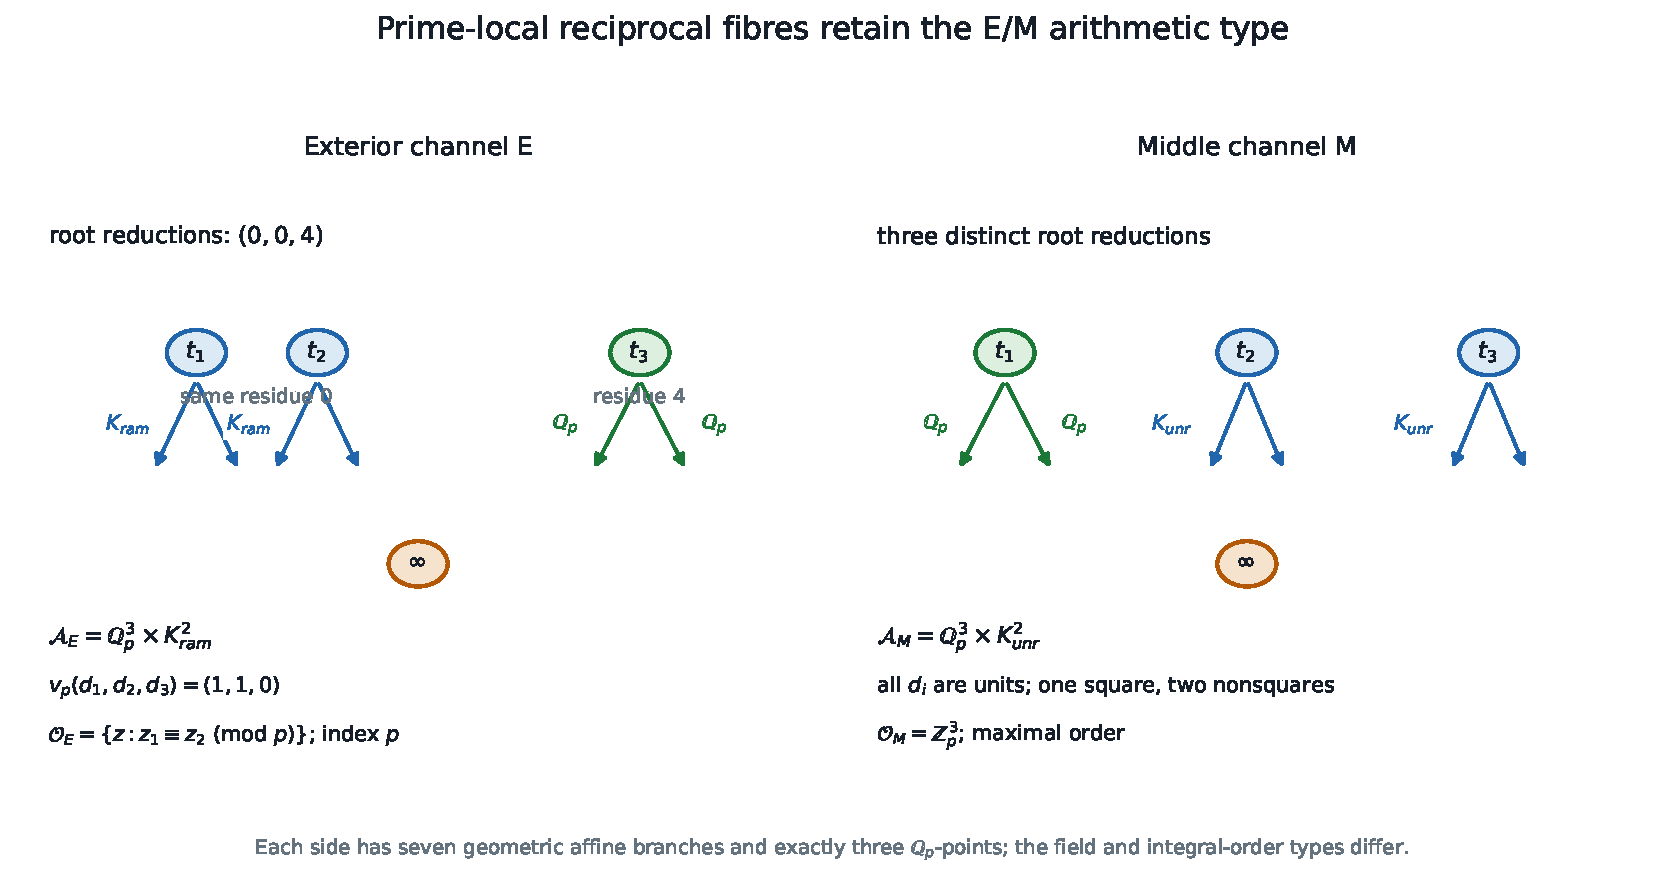
\includegraphics[width=.96\textwidth]{figures/prime-local-fibre-comparison.pdf}
\caption{The two complete prime-local fibre algebras.  Equal local-point
counts do not identify the ramified exterior and unramified middle factors,
and the exterior integral root order retains its exact index-\(p\) defect.}
\end{figure}

\begin{figure}[htbp]
\centering
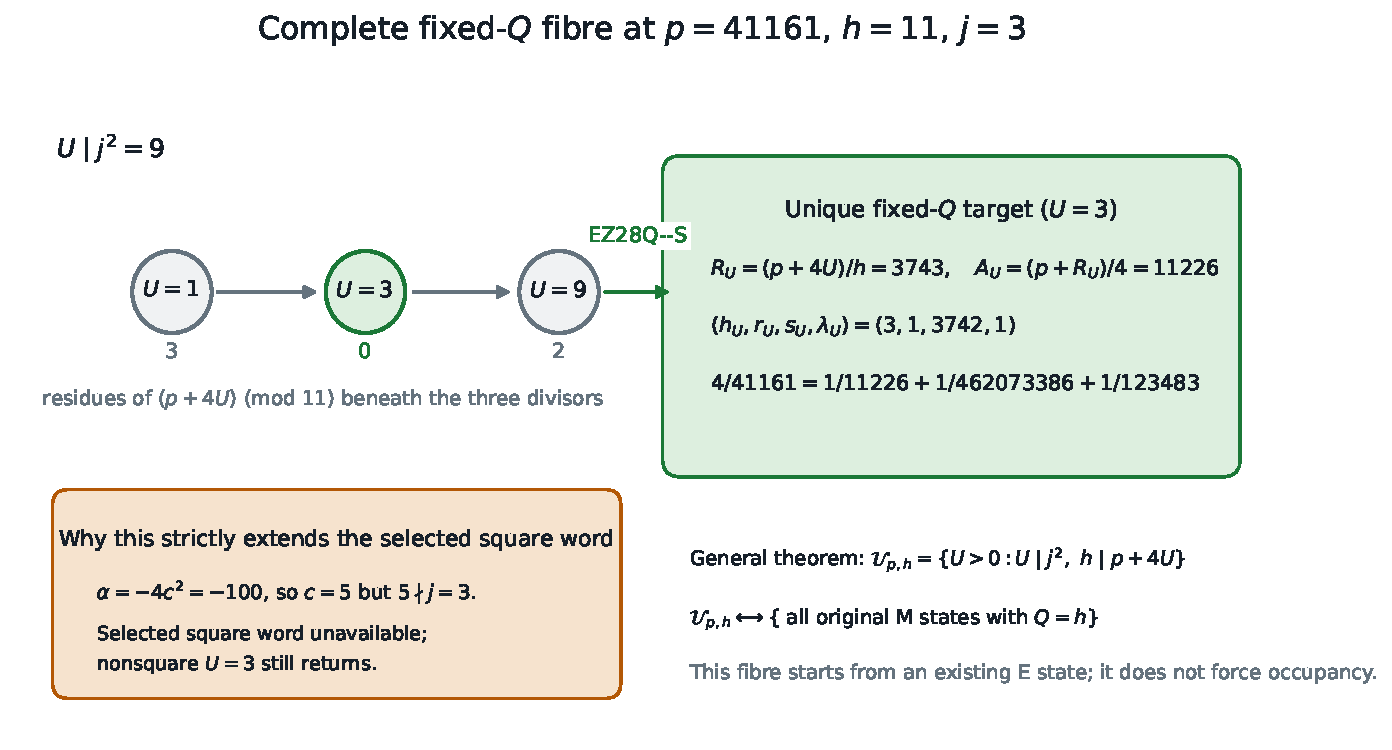
\includegraphics[width=.96\textwidth]{figures/fixed-q-fibre-41161.pdf}
\caption{At \(p=41161,h=11,j=3\), the complete divisor fibre contains the
nonsquare word \(U=3\), which gives the displayed middle witness although
the earlier selected square word is unavailable.}
\end{figure}

\begin{thebibliography}{9}
\small\raggedright
\bibitem{ET} Elsholtz, C., \& Tao, T. (2013). Counting the number of solutions
to the Erd\H{o}s--Straus equation on unit fractions. \emph{J. Aust. Math. Soc.,94},
50--105. \texttt{arXiv:1107.1010}, \S2.
\bibitem{Zeta} Split-Zero programme. (2026). \emph{The ES--Fable inverse
correspondence in the original weighted conductor}. GF1--11, GF16--18,
FC32--35. Zeta workbench revision \texttt{369f6ea9e0312bdf348ca9efd294735efc99c51d},
source blob \texttt{f777bb9f1434fa90f2f8bc762860048cc1d32bb4}.
The four-dimensional polynomial and inverse are antecedents, not newly claimed here.
\end{thebibliography}
\end{document}
